

\section{Paths in DAGs}\label{dp: sec: paths in DAGs}\doHeader{Paths in DAGs}

% \newcommand{\NODE}[1]{\text{point }{\small\ensuremath{(#1)}}\xspace}

\subsection{Counting Paths in a Grid}

Here's a toy problem to consider: \prob{Counting Paths in a Grid}.

\noindent\parbox{4in}{
  \begin{mylist}
  \item[\bf input:]
    Non-negative integers $i$ and $j$.

  \item[\bf output:]
    The number of paths from the origin $\NODE 0 0$ to the node $\NODE i j$ at location $(i, j)$
    in the 2D grid,  as illustrated to the right,
    assuming each step in the path moves one unit up or one unit to the right.
  \end{mylist}
}~~\parbox{2in}{
  \tikzset{
    dot/.style 2 args={fill, circle, inner sep=1pt, label={#1:\scriptsize #2}}
  }
  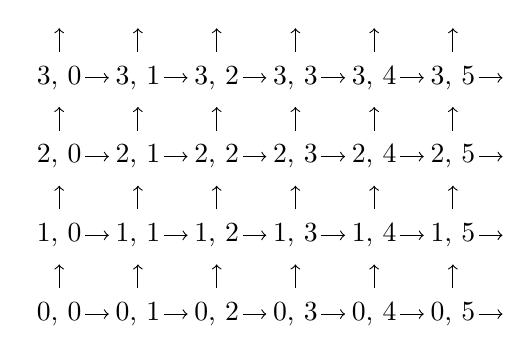
\begin{tikzpicture}
    \def\numberlist{{
      "0, 0","0, 1","0, 2","0, 3","0, 4","0, 5",
      "1, 0","1, 1","1, 2","1, 3","1, 4","1, 5",
      "2, 0","2, 1","2, 2","2, 3","2, 4","2, 5",
      "3, 0","3, 1","3, 2","3, 3","3, 4","3, 5"
      }}
    \def\maxX{5}
    \def\maxY{3}
    \foreach \x [count=\n] in {0,...,\maxX}{
      \foreach \y in {0,...,\maxY}{
        \pgfmathtruncatemacro\tmp{\n+(\maxX+1)*\y}
        \ifthenelse{\y=\maxY}{}{\draw[->] (\x,\y+0.33) -- (\x,\y+0.63);}
        \ifthenelse{\x=\maxX}{}{\draw[->] (\x+0.33,\y) -- (\x+0.63,\y);}
        % \node[shape=circle, draw=black, font=\small \sf] at (\x,\y) {\pgfmathparse{\numberlist[\tmp-1]}\pgfmathresult}; 
        \node[draw=none] at (\x, \y) {\NODEone{\pgfmathparse{\numberlist[\tmp-1]}\pgfmathresult}}; 
      }
    }
  \end{tikzpicture}
}

For example, how many paths are there from \NODE 0 0
% [review 2026-09-27] fix: the figure's top-right node is v_{3,5} (not v_{5,3}); changed the node and P(5,3) to (3,5)
to \NODE 3  5 in the graph to the right?
Let $P(i,j)$ denote the set of paths from \NODE 0 0 to \NODE i j.
We want to count the size of $P(3,5)$ (denoted $|P(3,5)|$).
The next lemma gives a divide-and-conquer approach:

\begin{lemma}\label{dp: lemma z} For $i, j \ge 0$,
  \(
    |P(i,j)| = \begin{cases}
      1 & \text{ if } i=0 \text{ or } j=0 \\
      |P(i,j-1)| + |P(i-1,j)| & \text{ otherwise }.
    \end{cases}
  \)
\end{lemma}
\begin{proof}
  When $i=0$ or $j=0$, the lemma holds because (by inspection of the grid) there is only one path.
  So assume $i>0$ and $j>0$.
  Partition the set $P(i,j)$ of paths from \NODE 0 0 to \NODE i j
  into two subsets:
  \begin{mylist}
  \item[(A)] The paths that enter $\NODE i j$  through $\NODE i {j-1}$.
  \item[(B)] The paths that enter  $\NODE i j$ through $\NODE {i-1} j$.
  \end{mylist}
  By inspection of the grid, every path into $\NODE i  j$
  enters either through  $\NODE i {j-1}$ or through  $\NODE {i-1} j$, 
  so the two subsets (A) and (B) partition $P(i,j)$.

  The number of paths entering $\NODE i j$ through $\NODE {i-1} j$
  equals the number of paths to $\NODE {i-1} j$,
  because each path to $\NODE {i-1} j$,
  followed by the edge from there to $\NODE i j$,
  yields a unique path into $\NODE i j$.
  Similarly, the number of paths entering $\NODE i j$ through $\NODE i {j-1}$
  equals the number of paths to $\NODE i {j-1}$.
\end{proof}

\newcommand{\countPaths}{\textsf{countPaths}}

The lemma gives this recursive algorithm for \prob{Counting Paths in a grid}:
\begin{myframed}
  \begin{steps}
  \item[]
    \countPaths$(i, j)$ \comment{--- return the number of paths from \NODE 0 0 to \NODE i j}
    \step return \(
      \begin{cases}
        1 & \text{ if } i = 0 \text{ or } j = 0
        \\
        \countPaths(i, j-1) + \countPaths(i-1, j)
        & \text{ otherwise }
      \end{cases}
    \)
  \end{steps}
\end{myframed}

\smallskip

There is one problem with this algorithm:
it takes time exponential in $i$ and $j$.
To see why, consider the recursion tree for $\countPaths(n, n)$.
In the tree, each leaf has depth at least $n$,
and each non-leaf node has two children,
so the number of nodes in each level $i\le n$ is $2^i$.
So executing $\countPaths(n,n)$ results in more than $2^n$ recursive calls altogether!

\paragraph{Two ways to avoid solving subproblems multiple times.}
In the execution of \countPaths$(i, j)$,
exponentially many recursive calls can arise.
But each recursive call that arises is of the form
\countPaths$(a, b)$ where $0\le a \le i$ and $0\le b\le j$.
And there are only $(i+1)\cdot (j+1)$ such pairs $(a,b)$
(one for each point lying to the left of and below point $(i, j)$).
So, the number of \emph{different} subproblems solved during the execution is only $\Theta(i\,j)$.

The reason that the recursive implementation above
takes exponential time is that \emph{it solves each distinct subproblem many times}.
You can see this by trying it out on the example,
or diagramming the recursion tree.
This redundancy is unnecessary.
\emph{It's enough to solve each distinct subproblem just once.}
There are two standard ways to do this.

\subsubsection{Memoizing}
\emph{Memoizing} caches the value returned by each call,
to avoid computing it again:

\smallskip 

\begin{myframed}
  \begin{steps}
  \item[]
    \countPaths$(i, j)$: \comment{--- return the number of paths from $(0,0)$ to $(i, j)$ in the 2d grid}

    \step maintain global ``cache'' array $C[]$, initially empty \smallskip

    \step if $C[i,j]$ has not previously been set:
    \comment{(store the value in the cache)}
    \smallskip
    \step~~~~~~~set \(C[i, j] = \begin{cases}
      1 & \text{ if } i = 0 \text{ or } j = 0
      \\
      \countPaths(i, j-1) + \countPaths(i-1, j)
      & \text{ otherwise }
    \end{cases}
    \)
    \step return $C[i, j]$
  \end{steps}
\end{myframed}

\smallskip 

Consider executing $\countPaths(i, j)$ with this modification.
Now, in the recursion tree, there will be just one non-leaf node
for each point $(a,b)$ with $0 < a \le i$ and $0 < b\le j$,
representing the first time $\countPaths(a, b)$ is called.
Subsequent calls with identical parameter values $(a,b)$ will return the cached value, without recursing.
So the total number of non-leaf nodes is $\Theta(i\,j)$.
And the number of leaf nodes is at most twice the number of non-leaf nodes
(since each non-leaf node has two children).
So the total number of nodes is also $\Theta(i\,j)$.
The work associated with each node is constant,
so the total time is $\Theta(i\,j)$, instead of exponential in $i$ and $j$.

\subsubsection{Iterating over the subproblems}
The second standard fix is to avoid recursion altogether, by simply iterating over the distinct subproblems:

\smallskip 

\begin{myframed}
  \begin{steps}
  \item[]\countPaths$(i, j)$:
    \comment{--- return the number of paths from $(0,0)$ to $(i,j)$ in the 2d grid}
    
    \step for $a=0,1,2,\ldots,i$: 
    \begin{block}
      \step~for $b=0,1,2,\ldots,j$: 
      \step~~~~~ \(N[a, b] = \begin{cases}
          1 & \text{ if } a = 0 \text{ or } b = 0
          \\
          N[a, b-1] + N[a-1, b] & \text{otherwise}
      \end{cases}\)
    \end{block}
    \step return $N[i, j]$
  \end{steps}
\end{myframed}

\smallskip 

With this approach, \emph{the iteration order matters!!!}
Each $N[a,b]$ must be computed \emph{after} $N[a,b-1]$ and $N[a-1, b]$.
This requirement is easy to satisfy for this problem,
but is more complicated to satisfy for some others.

With either approach, correctness of the resulting algorithm follows
by induction on the problem size and Lemma~\ref{dp: lemma z}.
This implementation requires (by inspection)  $\Theta(i\,j)$ additions,
but the values involved can be roughly as large as $2^{i+j}$,
so large-integer arithmetic on $(i+j)$-bit integers is required.
Then each addition takes time $O(i+j)$,
yielding the following theorem:
\begin{theorem}
  Given integers $i, j\ge 0$,
  we can compute, in $O((i+j)ij)$ time,
  the number of paths in the 2d grid graph (defined earlier)
  from the origin to $\NODE i j$.
\end{theorem}

\pythonCode{dynamic_programming/dynamic_programming_paths.py}

\newpage

\subsection{Shortest Path in a Grid}
The same reasoning easily extends to solve other problems on paths in a grid,
such as finding a shortest path.

\noindent
\parbox{4.2in}{
  \begin{mylist}
  \item[\bf input:]
    Non-negative integers $i$ and $j$, and a weight for each edge in the 2d grid graph.

  \item[\bf output:]
    The minimum, over all paths from $\NODE 0 0$ to $\NODE i j$,
    of the total weight of edges on the path.
  \end{mylist}

  To the right is the graph with some edge weights added (in blue).
}~~\parbox{2in}{
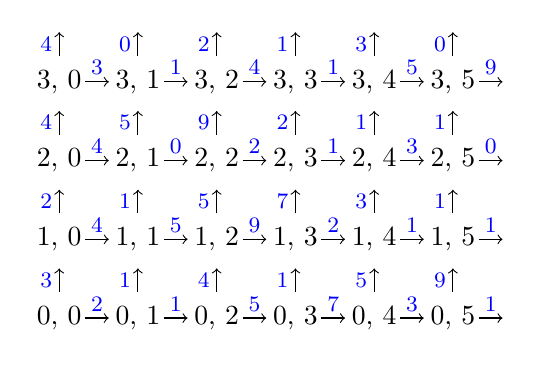
\begin{tikzpicture}
  \def\numberlist{{
      "0, 0","0, 1","0, 2","0, 3","0, 4","0, 5",
      "1, 0","1, 1","1, 2","1, 3","1, 4","1, 5",
      "2, 0","2, 1","2, 2","2, 3","2, 4","2, 5",
      "3, 0","3, 1","3, 2","3, 3","3, 4","3, 5"
    }}
  \def\edgelistA{{"3", "1", "4", "1", "5", "9", "2", "1", "5", "7", "3", "1", "4", "5", "9", "2", "1", "1", "4", "0", "2", "1", "3", "0"}}
  \def\edgelistB{{"2", "1", "5", "7", "3", "1", "4", "5", "9", "2", "1", "1", "4", "0", "2", "1", "3", "0", "3", "1", "4", "1", "5", "9"}}
  \def\maxX{5}
  \def\maxY{3}
  \foreach \x [count=\n] in {0,...,\maxX}{
    \foreach \y in {0,...,\maxY}{
      \pgfmathtruncatemacro\tmp{\n+(\maxX+1)*\y}
      \ifthenelse{\y=\maxY}{}{\draw[->] (\x,\y+0.33) -- (\x,\y+0.63)
        node [midway,left=-1pt,font=\color{blue}\footnotesize]
        {\pgfmathparse{\edgelistA[\tmp-1]}\pgfmathresult}; 
      }
      \ifthenelse{\x=\maxX}{}{\draw[->] (\x+0.33,\y) -- (\x+0.63,\y)
        node [midway,above=-1pt,font=\color{blue}\footnotesize]
        {\pgfmathparse{\edgelistB[\tmp-1]}\pgfmathresult};
      }
      % \node[shape=circle, draw=black, font=\small \sf] at (\x,\y) {\pgfmathparse{\numberlist[\tmp-1]}\pgfmathresult};
      \node[draw=none] at (\x, \y) {\NODEone{\pgfmathparse{\numberlist[\tmp-1]}\pgfmathresult}}; 
      }
    }
\end{tikzpicture}
}

Recall that $P(i, j)$ denotes the set of paths from \NODE0 0 to \NODE i  j.
Our goal now is to compute the minimum, over all paths in this set, of the total weight of edges in the path.

\smallskip

Define $M(i, j)$ to be this minimum weight.
Let $w(\NODE a b,\, \NODE c d)$
denote the weight of the edge from $\NODE a b$ to $\NODE c d$
(if the edge is present, that is, if $(c,d) = (a+1, b)$ or $(c,d) = (a, b+1)$).

\begin{lemma}\label{dp: lemma weight} For $i, j \ge 0$,
  \(
  M(i,j) = \begin{cases}
    0 & \text{ if } i=0 \text{ and } j=0,\\
    M(i-1, j)+ w(\NODE {i-1} j,\, \NODE i j) & \text{ if }i > 0 \text{ and } j=0, \\
    M(i, j-1)+ w(\NODE {i} {j-1},\, \NODE i j) & \text{ if } i=0  \text{ and } j > 0,\\
    \min\Big(\begin{array}{l}
      M(i-1, j)+ w(\NODE {i-1} j,\, \NODE i j), \\
      M(i, j-1)+ w(\NODE {i} {j-1},\, \NODE i j)
    \end{array}\Big)
    & \text{ if } i>0 \text{ and } j> 0.
  \end{cases}
  \)
\end{lemma}
\begin{proof}[Proof sketch.]
  When $i=0$ and $j=0$, the lemma holds because the only path is the empty path.

  Next we give the proof just for the case $i>0$ and $j>0$. (The remaining cases are easier.)
  As before, partition the set $P(i,j)$ of paths from \NODE 0 0 to \NODE i  j
  into two types:
  \begin{mylist}
  % [review 2026-09-27] fix: labels (A)/(B) were swapped relative to the proof body below (which derives M(i-1,j)+w for type (A)); swapped the two definitions
  \item[(A)] The paths that enter $\NODE i j$ from $\NODE {i-1} j$.
  \item[(B)] The paths that enter  $\NODE i j$ from $\NODE i {j-1}$.
  \end{mylist}
  By inspection of the grid, every path into $\NODE i  j$
  enters either through  $\NODE i {j-1}$ or through  $\NODE {i-1} j$, 
  so the two subsets (A) and (B) partition $P(i,j)$.
  It follows that the minimum weight of any path in $P(i,j)$
  is the minimum weight of any path of type (A), 
  or the minimum weight of any path of type (B),
  whichever is smaller.
  
  The paths of type (A) can be obtained by taking any path to $\NODE {i-1} j$ and adding
  the edge from $\NODE {i-1} j$ to $\NODE i j$.
  So the minimum weight of any path of type (A) 
  is the minimum weight of any path into $\NODE {i-1} j$,
  plus the weight of that edge.
  That is, the minimum weight of any type-(A) path
  is $M(i-1, j)+ w(\NODE {i-1} j,\, \NODE i j)$. 

  By similar reasoning, the minimum weight of any type-(B) path
  is $M(i, j-1)+ w(\NODE {i} {j-1},\, \NODE i j)$.

  It follows (when $i>0$ and $j>0$), that
  \(M(i, j) = 
    \min\Big(\begin{array}{l}
      M(i-1, j)+ w(\NODE {i-1} j,\, \NODE i j), \\
      M(i, j-1)+ w(\NODE {i} {j-1},\, \NODE i j)
    \end{array}\Big)
  \).
\end{proof}

\smallskip

Here is the resulting algorithm (the iterative implementation):

\newcommand{\shortestPath}{\textsf{shortestPath}}
\newcommand{\shortestPaths}{\textsf{shortestPaths}}

\begin{myframed}
  \begin{steps}
  \item[]\shortestPath$(i, j, w)$:
    \comment{--- return the minimum weight of any path from $\NODE 0 0$ to $\NODE i j$}

    \step for $a=0,1,2,\ldots,i$: 
    \begin{block}
      \step~for $b=0,1,2,\ldots,j$: 
      \step~~~~~\(M[a, b] = 
      \begin{cases}
        0 & \text{ if } a=0 \text{ and } b=0,\\
        M[a-1, b]+ w(\NODE {a-1} b,\, \NODE a b) & \text{ if }a > 0 \text{ and } b=0, \\
        M[a, b-1]+ w(\NODE {a} {b-1},\, \NODE a b) & \text{ if } a=0  \text{ and } b > 0,\\
        \min\begin{cases}
          M[a-1, b]+ w(\NODE {a-1} b,\, \NODE a b) \\
          M[a, b-1]+ w(\NODE {a} {b-1},\, \NODE a b)
        \end{cases}
        & \text{ if } a>0 \text{ and } b> 0.
      \end{cases}
      \)
    \end{block}
    \step return $M[i, j]$
  \end{steps}
\end{myframed}

\medskip 

Correctness of the algorithm follows from the lemma and induction on the problem size.

By inspection the algorithm runs in time $\Theta(i j)$.
This proves the following theorem:

\begin{theorem}
  Given integers $i, j\ge 0$ and edge weights for the 2d grid graph (defined earlier),
  we can compute, in $O(i\,j)$ time,
  the minimum weight of any path from the origin to $\NODE i j$.
\end{theorem}

% \continued

\subsection{\prob{Shortest Path in a DAG}}
The previous reasoning for grid graphs extends easily to any directed acyclic graph (DAG).
To illustrate this, consider finding shortest paths in an edge-weighted DAG:

\begin{mylist}
\item[\bf input:]
  DAG $G=(V,E)$ with edge weights; source vertex $s$, destination vertex $w$

\item[\bf output:]
  The shortest-path distance from $s$ to $w$
\end{mylist}
  
Fix any such input.
We start with the following recurrence relation:
\begin{lemma}\label{dp: lemma: DAGs} 
  For any vertex $w\in V$:
  \[
  \dist s w = \begin{cases}
    0 & \text{ if } w = s \\
    \min \big\{ \dist s u + \weight {u,w} : (u, w)\in E\big\}  & \text{ otherwise.}
  \end{cases}
  \]
\end{lemma}
\begin{proof}[Proof sketch.]
  In the case that $w=s$, the lemma holds because the only path is the empty path.

  Consider the case $w\ne s$.
  The shortest path from $s$ to $w$ is the shortest,
  over all possible edges $(u, w)$ into $w$,
  of the shortest among the paths ending in that edge $(u,w)$.
  Among the paths from $s$ to $w$ ending in a given edge $(u, w)$,
  a shortest one can be obtained by taking any shortest path from $s$ to $u$, and appending edge $(u,w)$.
  Hence the shortest path from $s$ to $w$ ending in $(u,w)$
  has weight $\dist s u  + \weight {u, w}$.
\end{proof}

This gives the following recursive algorithm:

\begin{myframed}
  \begin{steps}
  \item[]\shortestPath$(G=(V,E), s, w)$:
    \comment{return the shortest-path distance from $s$ to $w$ in DAG $G$}

    \step~~~return
    \(\begin{cases}
      0 & \text{ if } w = s \\
      % [review 2026-09-27] fix: the recursive call dropped the graph argument G; changed shortestPath(s,u) to shortestPath(G,s,u)
      \min \big\{ \shortestPath(G, s, u) + \weight {u,w}: (u, w)\in E\big\}  & \text{ otherwise.}
    \end{cases}\)
  \end{steps}
\end{myframed}

% [review 2026-09-27] fix: the empty-min = infinity convention was stated only for the iterative version; stated it for the recursive version too
If $w$ has no in-neighbors, so the set is empty, the minimum has value $\infty$.

Correctness follows from Lemma~\ref{dp: lemma: DAGs} and induction.
(Show by induction on the recursion depth
that \shortestPath$(G, s, w) = \dist s w$ for all $w\in V$.)
We memoize the algorithm.  Then the recursion tree will have
at most one non-leaf node for each vertex $v\in V$,
and the work associated with that node will be proportional to the in-degree of $v$
(the number of edges into $v$),
so the total time will be $\Theta(n+m)$.

If we want instead an iterative algorithm, we have to explicitly compute an order
in which to evaluate the subproblems.  We can only evaluate a given subproblem
$\shortestPath(G, s, w)$
\emph{after}
the subproblem for each in-neighbor $u$ of $w$ is done.
This is exactly what topological ordering is for!
The algorithm first computes a topological ordering of the vertices
(in linear time using DFS, as described in \LN{graphs}),
then considers the vertices in that order.

\begin{myframed}
  \begin{steps}
  \item[]\shortestPath$(G=(V,E), s, w)$:
    \comment{return the shortest-path distance from $s$ to $w$ in DAG $G$}

    \step let $v_1, v_2, \ldots, v_n$ be a topological ordering of the vertices (computed using DFS; see \LN{graphs})
    
    \step for $j=1,2,\ldots, n$:

    \step~~~~set \(d[v_j] = 
    \begin{cases}
      0 & \text{ if } v_j = s \\
      \min \big\{ d[v_i] + \weight {v_i,v_j}: (v_i, v_j)\in E\big\}  & \text{ otherwise.}
    \end{cases}
    \)

    \step return $d[w]$
    
  \end{steps}
\end{myframed}

In Step 3 if $v_j$ has no in-neighbors, so the set is empty, the minimum has value $\infty$.

Correctness follows from Lemma~\ref{dp: lemma: DAGs} and induction. 
(Show by induction on $j$ that
that $d[v_j] = \dist s {v_j}$ for all $j\in\{1,2,\ldots,n\}$.)
The time to evaluate the right-hand side in Step 3 is $\Theta(1+\text{in-degree}(v_j))$.
Summing over all the vertices,
the total time is $\Theta(n+m)$.
We conclude with a theorem that summarizes what we've figured out:
\begin{theorem}
  There is a linear-time algorithm for \prob{Shortest Path in a DAG}.
\end{theorem}

\pythonCode{dynamic_programming/dynamic_programming_paths.py}

\exercise\emph{(implementation)}
Implement the algorithm and test your implementation on Hackerrank.com, at
\url{https://www.hackerrank.com/nealeyoung-algs101-dag-paths-and-topological-sort}
(the ``Shortest-path distances in a DAG'' challenge; there, edge weights can be negative).

\solution
\pythonCode{dynamic_programming/dynamic_programming_paths.py}

\subsection{\prob{Longest Path in a DAG}}

The same reasoning yields a linear-time algorithm for \prob{Longest Path in a DAG}
(computing the \emph{maximum} weight of any path from $s$ to $w$).
The algorithm and its derivation are exactly the same as for \prob{Shortest Path in a DAG},
but each ``$\min$'' is replaced by a ``$\max$''.
We leave the details as an exercise. 

\pythonCode{dynamic_programming/dynamic_programming_paths.py}

% \subsection*{External sources on Shortest Paths in a DAG}

% \begin{itemize}
% \item \JE Section 8.5; DPV Section 4.7; CLRS Section 24.2.
% \end{itemize}


%%% Local Variables:
%%% mode: latex
%%% TeX-master: "dynamic_programming"
%%% End:
